\documentclass[10pt,a4paper]{article}

\usepackage[a4paper,top=18mm,bottom=18mm,left=18mm,right=18mm]{geometry}
\usepackage[T1]{fontenc}
\usepackage{lmodern,microtype}
\usepackage{amsmath,amssymb,mathtools,bm}
\usepackage{xcolor,booktabs,tabularx,array,enumitem,multicol,graphicx}
\usepackage{tikz}
\usetikzlibrary{arrows.meta,positioning,calc}
\usepackage[most]{tcolorbox}
\usepackage{fancyhdr,hyperref}
\definecolor{ink}{HTML}{24354B}
\definecolor{accent}{HTML}{135E77}
\definecolor{pale}{HTML}{F1F7F8}
\hypersetup{colorlinks=true,linkcolor=accent,urlcolor=accent,pdfauthor={PHYS4055 revision notes}}
\setlength{\parindent}{0pt}
\setlength{\parskip}{4pt}
\setlength{\emergencystretch}{3em}
\setlist{leftmargin=*,topsep=2pt,itemsep=1pt}
\AtBeginDocument{\color{ink}}
\pagestyle{fancy}
\fancyhf{}
\fancyhead[L]{\footnotesize PHYS4055 \textbar\ Exam Revision}
\fancyhead[R]{\footnotesize 2026 \textbar\ Open-book notes}
\fancyfoot[C]{\footnotesize\thepage}
\renewcommand{\headrulewidth}{0.3pt}
\newcommand{\ket}[1]{\left\lvert #1\right\rangle}
\newcommand{\bra}[1]{\left\langle #1\right\rvert}
\newcommand{\braket}[2]{\left\langle #1\middle\vert #2\right\rangle}
\newcommand{\mel}[3]{\left\langle #1\middle\vert #2\middle\vert #3\right\rangle}
\newcommand{\diff}{\mathrm{d}}
\newcommand{\ii}{\mathrm{i}}
\newcommand{\e}{\mathrm{e}}
\newtcolorbox{methodbox}{colback=pale,colframe=accent!50!white,boxrule=0.4pt,arc=1mm,before skip=5pt,after skip=5pt}
\newtcolorbox{cautionbox}{colback=white,colframe=black!20,boxrule=0.4pt,arc=1mm,before skip=5pt,after skip=5pt}

\usepackage{titlesec}
\geometry{top=16mm,bottom=16mm,left=17mm,right=17mm,headsep=5mm,footskip=7mm}
\hypersetup{pdftitle={PHYS4055 2023-2025 Complete Worked Past Exam Solutions}}
\setlength{\parskip}{3pt plus 1pt minus .2pt}
\setlength{\emergencystretch}{3em}
\renewcommand{\arraystretch}{1.18}
\titleformat{\section}{\large\bfseries\color{accent}}{\thesection}{.6em}{}
\titlespacing*{\section}{0pt}{13pt plus 2pt}{7pt}
\newcommand{\examquestion}[4]{%
\section[#1 Q#2]{Question #2: #3}%
{\footnotesize\color{gray}Original: PHYS4055 Semester 2 #1,
Question #2, source paper page #4. All subparts answered.}\par\vspace{3pt}}
\newcommand{\solcheck}[1]{\begin{methodbox}\footnotesize
\textbf{Verification check.} #1\end{methodbox}}
\newcommand{\paperyear}[1]{\clearpage
\phantomsection
\addcontentsline{toc}{part}{#1 examination}
\begin{center}{\color{accent}\LARGE\bfseries
Semester 2 #1 examination}\end{center}
\vspace{2pt}\hrule\vspace{7pt}}
\begin{document}
\begin{center}
\vspace*{8mm}
{\Huge\bfseries\color{accent}PHYS4055}\\[4mm]
{\LARGE Atomic Physics and Quantum Optics}\\[7mm]
{\Large\bfseries Complete Worked Past Exam Solutions}\\[4mm]
{\Large 2023 \(\cdot\) 2024 \(\cdot\) 2025}\\[5mm]
{\normalsize All 12 questions, including every subpart}\\[4mm]
{\normalsize 2026 open-book examination preparation}
\end{center}
\vspace{8mm}
\begin{methodbox}
\textbf{What this book contains.}
All four questions from \emph{each} of the three
uploaded exam papers are solved step by step.
The calculations include intermediate algebra,
physical reasoning, level sketches and result
checks. Although the papers require students
to answer only three of four questions, this
book covers \emph{every} question.
\end{methodbox}
\noindent{\bfseries How to use it:}
Read a past question first, attempt the
derivation, then compare the worked steps.
For a timed revision exercise, choose
three questions per paper and work for two hours.
\begin{cautionbox}
\textbf{Important conventions and source caveats.}
The original PDFs in \texttt{source\_material/past\_exams}
remain authoritative for diagrams and printed notation.
When a problem leaves a speed convention or squeezed-state
ordering unspecified, this book states a reasonable convention
and also notes valid alternatives. In the 2024 sensor
problem a dimensionally necessary \(\kappa\) factor is
derived explicitly. These are independently prepared
study solutions; no official past-exam marking scheme
was provided.
\end{cautionbox}
\vspace{4mm}
\begin{center}\small
\begin{tabularx}{\linewidth}{@{}lX@{}}
\toprule
\textbf{Paper}&\textbf{Question themes}\\\midrule
2023&
Nonlinear optical cat states; H/He radial and spin structure;
squeezed interferometry; Raman \(\pi\)-pulse sensing\\
2024&
\({}^3D\) spin--orbit splitting; Zeeman sensor;
HOM and statistics; lossy cavity and dual-rail gates\\
2025&
Hyperfine/Zeeman structure; Yb optical clock, cooling
and Doppler limit; NOON-state beam splitter;
parametric cavity squeezing and Bell keys\\
\bottomrule
\end{tabularx}
\end{center}
\vfill
{\footnotesize First prepared 13 November 2026.
Source audit: \texttt{SOURCE\_MAP.md}.
Editable sections: \texttt{sections/\{year\}\_q\{n\}.tex}.}
\clearpage
\tableofcontents

\paperyear{2023}

\examquestion{2023}{1}{A nonlinear optical mode: coherent states and Schr\"odinger cats}{2}
Consider the Hamiltonian
\[
H=\hbar[\omega a^\dagger a+\lambda(a^\dagger a)^p]
=\hbar[\omega\hat n+\lambda\hat n^p].
\]
Take \(p\) to be a \emph{positive} integer and
\(\lambda\ne0\) in the specified evolution time.

\subsection*{(a) Eigenstates and eigenvalues}
Because \(H\) is a function of \(\hat n=a^\dagger a\),
all number states are eigenstates:
\[
\boxed{H\ket n=E_n\ket n,\qquad
E_n=\hbar(\omega n+\lambda n^p),\quad n=0,1,2,\ldots}.
\]
This is a number-dependent nonlinearity. The
energy spacings are generally not constant.

\subsection*{(b) Evolve a coherent input in the interaction picture}
Take \(H_0=\hbar\omega\hat n\); it commutes with
\(H_I=\hbar\lambda\hat n^p\).
Write the initial coherent state as
\[
\ket\alpha=e^{-|\alpha|^2/2}
\sum_{n=0}^\infty\frac{\alpha^n}{\sqrt{n!}}\ket n .
\]
Since
\(U_I(t)=\exp(-i\lambda t\hat n^p)\),
the evolved state is
\[
\boxed{\ket{\psi_I(t)}=
e^{-|\alpha|^2/2}
\sum_{n=0}^\infty
\frac{\alpha^n}{\sqrt{n!}}
e^{-i\lambda t n^p}\ket n}.
\]
The nonlinear unitary changes phases but
\emph{not} photon-number probabilities.

\subsection*{(c) Recover the coherent-state cat for even \(p\)}
For \(p=2,4,\ldots\) and integer \(n\),
\(n^p\) is divisible by 4 if \(n\) is even,
while \(n^p\equiv1\pmod4\) if \(n\) is odd.
At the time \(t=\pi/(2\lambda)\),
\[
e^{-i\pi n^p/2}=
\begin{cases}1,&n\text{ even},\\-i,&n\text{ odd}.\end{cases}
\]
The parity-dependent coefficient is
\[
e^{-i\pi n^p/2}=
\tfrac12[(1-i)+(1+i)(-1)^n].
\]
Substitute into the Fock expansion and use
\((-1)^n\alpha^n=(-\alpha)^n\):
\[
\boxed{\ket{\psi_I}=\frac12
[(1-i)\ket\alpha+(1+i)\ket{-\alpha}]}.
\]
It is correctly normalised: the cross term
between \(\ket\alpha\) and \(\ket{-\alpha}\)
has purely imaginary coefficient, while
\(\braket{\alpha}{-\alpha}=e^{-2|\alpha|^2}\)
is real.

\subsection*{(d) Calculate all normal-ordered correlations}
The diagonal photon-number probabilities remain
\[
P_n=e^{-|\alpha|^2}\frac{|\alpha|^{2n}}{n!}.
\]
For positive integer \(k\), the normally
ordered factorial moment is
\[
\langle(a^\dagger)^ka^k\rangle
=\sum_{n=k}^\infty
n(n-1)\cdots(n-k+1)P_n=|\alpha|^{2k}.
\]
As \(\langle\hat n\rangle=|\alpha|^2\),
\[
\boxed{g^{(k)}(0)=
\frac{\langle(a^\dagger)^ka^k\rangle}{
\langle\hat n\rangle^k}=1
\qquad(k=1,2,\ldots,\ |\alpha|>0).}
\]
This is the usual \emph{normalised zero-delay}
intensity-correlation definition.

\subsection*{(e) Is the state classical?}
Despite having \emph{Poissonian photon statistics}
and \(g^{(k)}(0)=1\), the state is a coherent
superposition of distinguishable field amplitudes
\(\alpha\) and \(-\alpha\), not a classical mixture.
Its phase-space representation contains quantum
interference fringes and, for nonzero well-resolved
amplitudes, Wigner negativity; a positive classical
mixture of coherent states cannot reproduce it.
Photon counts alone fail to reveal these
phase-sensitive coherences. For \(\alpha=0\) the
state reduces to the vacuum (not a nontrivial cat).
\solcheck{The relative phase between Fock amplitudes
changes, but \(|e^{-i\lambda tn^p}|^2=1\),
so every photon-number probability is unchanged.}


\examquestion{2023}{2}{Hydrogen radial probabilities, helium spins and E1 lines}{3}
The hydrogen \(1s\) wavefunction is
\[
\psi_{1s}(r)=\frac{e^{-r/a_0}}{\sqrt{\pi a_0^3}},
\qquad
|\psi_{1s}|^2=\frac{e^{-2r/a_0}}{\pi a_0^3}.
\]

\subsection*{(a) Radius with maximum detection probability}
The correct \emph{radial probability distribution}
is the probability in a spherical shell,
\(P(r)\diff r=4\pi r^2|\psi|^2\diff r\):
\[
P(r)=\frac{4r^2}{a_0^3}e^{-2r/a_0}.
\]
Differentiating the log,
\(P'/P=2/r-2/a_0\). Apart from the zero
endpoint, the maximum is
\[
\boxed{r_{\rm most\ probable}=a_0}.
\]
Maximising \(|\psi(r)|^2\) alone would wrongly give
\(r=0\): it omits the increasing spherical-shell volume.

\subsection*{(b) Evaluate \(\langle r\rangle\) and
\(\langle1/r\rangle\)}
Using
\(\int_0^\infty r^n e^{-\beta r}\diff r
=n!/\beta^{n+1}\),
\begin{align*}
\langle r\rangle
&=\frac4{a_0^3}\int_0^\infty
r^3e^{-2r/a_0}\diff r
=\frac4{a_0^3}\frac{3!}{(2/a_0)^4}
=\boxed{\frac{3a_0}{2}},\\
\left\langle\frac1r\right\rangle
&=\frac4{a_0^3}\int_0^\infty
re^{-2r/a_0}\diff r
=\frac4{a_0^3}\frac{1!}{(2/a_0)^2}
=\boxed{\frac1{a_0}}.
\end{align*}
Bohr's \(n=1\) orbit has fixed radius \(a_0\);
it agrees with the quantum \emph{most probable}
radius and \(\langle1/r\rangle=1/a_0\),
but not the mean radius \(\langle r\rangle=3a_0/2\).

\subsection*{(c) Schr\"odinger equation for helium}
For a fixed nucleus \(Z=2\), a simplified
non-relativistic two-electron Hamiltonian is
\[
\boxed{H=
-\frac{\hbar^2}{2m_e}(\nabla_1^2+\nabla_2^2)
-\frac{2e^2}{4\pi\epsilon_0}
\left(\frac1{r_1}+\frac1{r_2}\right)
+\frac{e^2}{4\pi\epsilon_0r_{12}}.}
\]
The three terms represent electron kinetic
energy, attractions to the nucleus and mutual
electron repulsion, respectively. Solve
\(H\Psi(\mathbf r_1,\mathbf r_2)=E\Psi\)
with total fermion-exchange antisymmetry.
Spin and relativistic interactions would be
additional smaller corrections.

\subsection*{(d) All four two-electron spin states}
\[
\begin{array}{c|l|c}
\text{Total }S&\text{Spin state}&\text{Exchange}\\\hline
1,\ M_S=1&\ket{\uparrow\uparrow}&\text{symmetric}\\
1,\ M_S=0&
(\ket{\uparrow\downarrow}+\ket{\downarrow\uparrow})/\sqrt2&
\text{symmetric}\\
1,\ M_S=-1&\ket{\downarrow\downarrow}&\text{symmetric}\\
0,\ M_S=0&
(\ket{\uparrow\downarrow}-\ket{\downarrow\uparrow})/\sqrt2&
\text{antisymmetric}
\end{array}
\]
The first three are the triplet, the last the singlet.
Since total two-electron wavefunction is antisymmetric,
a triplet needs an antisymmetric spatial part, while
a singlet needs a symmetric spatial part.

\subsection*{(e) Physical origin and relative magnitude of hyperfine structure}
Fine structure primarily concerns electronic
spin--orbit and relativistic effects. Hyperfine
structure couples electronic angular momentum and
fields to \emph{nuclear} magnetic dipole/electric
quadrupole moments. The nuclear magnetic moment
is typically of nuclear-magneton scale,
\(\mu_N=e\hbar/(2m_p)\), much smaller than the
electron Bohr magneton \(\mu_B=e\hbar/(2m_e)\);
this suppresses hyperfine interactions.
For \({}^4\mathrm{He}\), whose nucleus has \(I=0\),
magnetic-dipole hyperfine splitting is absent.

\subsection*{(f) Allowed E1 transitions among the stated terms}
To leading order in LS coupling, E1 requires
opposite orbital parity, \(\Delta S=0\), and
\(|\Delta J|\le1\) with \(J=0\not\to J'=0\).
Thus the allowed combinations are
\[
\boxed{{}^1P_1\longleftrightarrow{}^1S_0,\qquad
{}^3P_{0,1,2}\longleftrightarrow{}^3S_1.}
\]
The direction of spontaneous emission is from the
higher to the lower member of each pair.
Singlet--triplet lines are spin-forbidden in pure
LS coupling but can gain weak intensity through
spin--orbit mixing. A simple term diagram is:
\[
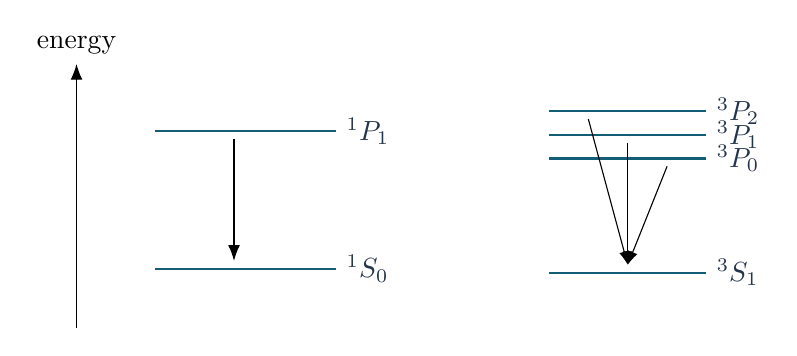
\begin{tikzpicture}[x=1cm,y=.5cm]
\draw[-{Latex[length=2mm]}](0,0)--(0,6.7) node[above]{energy};
\draw[accent,thick](1,5)--(3.3,5) node[right,ink]{\({}^1P_1\)};
\draw[accent,thick](1,1.5)--(3.3,1.5) node[right,ink]{\({}^1S_0\)};
\draw[-{Latex[length=2mm]}](2,4.8)--(2,1.7);
\draw[accent,thick](6,5.5)--(8,5.5) node[right,ink]{\({}^3P_2\)};
\draw[accent,thick](6,4.9)--(8,4.9) node[right,ink]{\({}^3P_1\)};
\draw[accent,thick](6,4.3)--(8,4.3) node[right,ink]{\({}^3P_0\)};
\draw[accent,thick](6,1.4)--(8,1.4) node[right,ink]{\({}^3S_1\)};
\foreach \y/\x in {5.5/6.5,4.9/7,4.3/7.5}
{\draw[-{Latex[length=1.7mm]}](\x,\y-.2)--(7,1.6);}
\end{tikzpicture}
\]
\solcheck{Radial expectations require the
\(4\pi r^2\) measure. For selection rules,
check \emph{spin}, \emph{parity} and \emph{angular
momentum} independently.}


\examquestion{2023}{3}{Squeezed-coherent input in a Mach--Zehnder interferometer}{4}
We have one squeezed-coherent input mode \(a\) and
one vacuum input mode \(v\).
For clarity, distinguish \emph{field displacement}
\(\alpha\) from squeeze parameters
\(\mu=\cosh r,\ \nu=e^{2i\varphi_S}\sinh r\).

\subsection*{(a) Energy conservation at the first beam splitter}
The stated beam splitter matrix is
\[
M=\frac1{\sqrt2}\begin{pmatrix}1&i\\i&1\end{pmatrix}.
\]
The input column of field amplitudes is
\(\mathbf E_{\rm in}=(E_{\rm in},E_v)^T\).
Since
\[
M^\dagger M=\frac12
\begin{pmatrix}1&-i\\-i&1\end{pmatrix}
\begin{pmatrix}1&i\\i&1\end{pmatrix}=I,
\]
we obtain
\[
\boxed{|E_1|^2+|E_2|^2=
\mathbf E_{\rm in}^\dagger M^\dagger M
\mathbf E_{\rm in}
=|E_{\rm in}|^2+|E_v|^2}.
\]
For quantum modes the analogous statement is
conservation of total photon number,
because \(M\) is unitary.

\subsection*{(b) Will squeezing enhance the sensitivity?}
Not \emph{automatically}. Squeezing can lower
noise in a selected quadrature, but the effect
depends on which input port is squeezed, its
squeezing angle, the operating phase and the
measurement. In this question the \emph{other input
is vacuum} and the measured observable is
the \emph{output photon-number difference}.
As the calculations below show, at \(\phi=\pi/2\)
the variance of the difference is the
\emph{mean photon number} of the occupied input.
Thus this exact configuration does \emph{not}
give sub-shot-noise phase resolution at fixed
total mean photon number through simple
difference detection. Injecting appropriately
squeezed vacuum in the unused port is a different
well-known enhancement scheme.

\subsection*{(c) Derive the number-difference operator}
The problem gives
\[
a_A=c\,a+d\,v,\qquad a_B=d\,a+c\,v,\quad
c=\tfrac12(e^{i\phi}+1),\quad
d=\tfrac12(e^{i\phi}-1).
\]
Compute the coefficients:
\[
|c|^2-|d|^2=\cos\phi,\qquad
c^*d-d^*c=i\sin\phi.
\]
Expand \(a_A^\dagger a_A-a_B^\dagger a_B\):
\[
\boxed{D\equiv n_A-n_B
=\cos\phi(n_a-n_v)
+i\sin\phi(a^\dagger v-v^\dagger a)}.
\]

\subsection*{(d) Signal for the squeezed-coherent input}
Since the second mode is vacuum,
\(\langle n_v\rangle=0\),
\(\langle v\rangle=0\); all cross-mode
expectation values factor. Hence
\[
\boxed{\langle D\rangle=\cos\phi\,N},
\qquad N=\langle a^\dagger a\rangle.
\]
For the conventional displaced-squeezed
state \(\ket{\alpha,\xi}=D(\alpha)S(\xi)\ket0\),
we have
\[
S^\dagger a S=\mu a-\nu a^\dagger,\qquad
\boxed{N=|\alpha|^2+|\nu|^2
=|\alpha|^2+\sinh^2 r}.
\]
Therefore
\[
\boxed{\langle n_A-n_B\rangle
=\cos\phi(|\alpha|^2+|\nu|^2)}.
\]
If the problem instead defines
\(\ket{\alpha,\xi}=S(\xi)D(\alpha)\ket0\),
operator ordering changes the number expectation:
\(N=|\mu\alpha-\nu\alpha^*|^2+|\nu|^2\).
The subsequent noise formula in terms of \(N\)
remains valid. \emph{State the convention.}

\subsection*{(e) Number-difference variance at \(\phi=\pi/2\)}
At the operating phase,
\(D=i(a^\dagger v-v^\dagger a)\) and
\(\langle D\rangle=0\). Square it:
\[
D^2=-a^\dagger v a^\dagger v
+a^\dagger v v^\dagger a
+v^\dagger a a^\dagger v
-v^\dagger a v^\dagger a.
\]
In the vacuum \(v\),
\(\langle v^\dagger v\rangle=0\),
\(\langle vv^\dagger\rangle=1\),
\(\langle v^2\rangle=\langle v^{\dagger2}\rangle=0\).
Only the second term remains, so
\[
\boxed{\operatorname{Var}(D)|_{\pi/2}
=\langle D^2\rangle
=\langle a^\dagger a\rangle=N
=|\alpha|^2+|\nu|^2}
\]
for \(D(\alpha)S(\xi)\ket0\).

\subsection*{(f) Minimum resolvable phase near \(\pi/2\)}
For a small deviation \(\epsilon\),
\(\cos(\pi/2+\epsilon)\simeq-\epsilon\).
Thus the signal magnitude is
\(|\langle D\rangle|\simeq N|\epsilon|\),
and the noise standard deviation is \(\sqrt N\).
Demanding signal-to-noise ratio 1 gives
\[
1\simeq\frac{N|\epsilon|}{\sqrt N},
\qquad
\boxed{\delta\phi_{\rm min}\simeq\frac1{\sqrt N}
=\frac1{\sqrt{|\alpha|^2+\sinh^2 r}}}.
\]
For \(M\) independent repetitions,
the standard error scales as \(1/\sqrt{MN}\).
Squeezing can raise \(N\) if \(\alpha\) is
held fixed, but \emph{at equal total photon
number} this is still shot-noise scaling.
\solcheck{The sensitivity must be computed using
the \emph{slope} at the dark operating point:
the mean signal itself is zero exactly at
\(\phi=\pi/2\). The derivation does not assume
a Gaussian input; only that the other port is vacuum.}


\examquestion{2023}{4}{Raman transition, atomic Bloch equations and pulse-area sensing}{5--6}
The question describes an effective two-photon
Raman coupling between \(\ket g,\ket e\)
mediated by an auxiliary state \(\ket a\).
The effective Hamiltonian is already written
in terms of a cavity photon and a control field;
the off-resonant auxiliary state has been
eliminated in the model.

\subsection*{(a) Remove the fast free oscillations}
Write
\[
\sigma_+=\ket e\bra g,\quad
\sigma_-=\ket g\bra e,\quad
H_0=\hbar\omega_a a^\dagger a+
\frac{\hbar\omega_{eg}}2\sigma_z.
\]
The interaction in the Schr\"odinger picture
contains
\(\hbar g\mathcal E_c(t)
a^\dagger\sigma_-e^{-i\omega_ct}+\mathrm{h.c.}\).
Under the free interaction picture,
\[
a^\dagger\sigma_-\mapsto
a^\dagger\sigma_-e^{i(\omega_a-\omega_{eg})t},
\]
so the coupling acquires
\[
e^{i(\omega_a-\omega_{eg}-\omega_c)t}
=e^{-i\delta t},
\quad \delta=\omega_{eg}-(\omega_a-\omega_c).
\]
A further rotating-frame phase transformation
transfers this time-dependent phase to the
cavity-number term. With a real control
envelope, an equivalent form is
\[
\boxed{H_I=-\hbar\delta\,a^\dagger a+
\hbar g\mathcal E_c(t)(a^\dagger\sigma_-+
a\sigma_+)}.
\]
The sign of the displayed number term is set
by the selected rotating-frame convention;
the physics depends on the \emph{relative}
two-photon detuning.

\subsection*{(b) Derive the equations for \(z,w\)}
For a strongly driven cavity mode replace
\(a\to\alpha\), \(a^\dagger\to\alpha^*\), treating
\(\alpha\) as the effective coherent amplitude
(including any detuning response).
The atomic coupling is
\(H_{\rm at}=\hbar g\mathcal E_c(t)
(\alpha^*\sigma_-+\alpha\sigma_+)\).
With
\[
z=\langle\sigma_z\rangle,\quad
w=\langle\sigma_+\rangle,\quad
w^*=\langle\sigma_-\rangle,
\]
and commutators
\([\sigma_z,\sigma_\pm]=\pm2\sigma_\pm\),
\([\sigma_-,\sigma_+]=-\sigma_z\),
the Heisenberg equation gives
\[
\dot z=\frac i\hbar\langle[H_{\rm at},\sigma_z]\rangle
=\boxed{2ig\mathcal E_c(t)(\alpha^*w^*-\alpha w)},
\]
\[
\dot w=\frac i\hbar
\langle[H_{\rm at},\sigma_+]\rangle
=\boxed{-ig\mathcal E_c(t)\alpha^* z}.
\]
Its conjugate is
\(\dot w^*=ig\mathcal E_c(t)\alpha z\).
The equations supplied in part (b) assume
that the coupling phase can be taken
time-independent in this rotating description.

\subsection*{(c) Pulse-area solution for complete inversion}
The specified envelope is
\(\mathcal E_c(t)=\mathcal E_0e^{-\gamma|t|}\).
The \emph{pulse area} is
\[
\boxed{\mathcal A=
\int_{-\infty}^\infty\mathcal E_c(t)\diff t
=\frac{2\mathcal E_0}{\gamma}}.
\]
Define the new time coordinate
\(\tau(t)=\int_{-\infty}^t\mathcal E_c(t')\diff t'\).
Then \(\diff/\diff t=\mathcal E_c(t)\diff/\diff\tau\).
The equations reduce to
\[
\frac{\diff z}{\diff\tau}
=2ig(\alpha^*w^*-\alpha w),\qquad
\frac{\diff w}{\diff\tau}=-ig\alpha^*z.
\]
Differentiate \(z\) once more and substitute
the equations for \(w,w^*\):
\[
\frac{\diff^2z}{\diff\tau^2}
=2ig[
\alpha^*(ig\alpha z)-\alpha(-ig\alpha^*z)]
=\boxed{-4g^2|\alpha|^2z}.
\]
The initial atom is in \(\ket g\), so
\(z(-\infty)=-1\), \(w(-\infty)=0\).
The resonant solution is
\[
\boxed{z(t)=-\cos[2g|\alpha|\tau(t)]},\quad
P_e(t)=\frac{1+z(t)}2
=\sin^2[g|\alpha|\tau(t)].
\]
After the complete pulse,
\[
\boxed{P_e(\infty)
=\sin^2\!\left(\frac{2g|\alpha|\mathcal E_0}{\gamma}\right)}.
\]
Complete population inversion requires
\[
\boxed{\frac{4g|\alpha|\mathcal E_0}{\gamma}
=(2m+1)\pi,\quad m=0,1,\ldots,}
\]
equivalently \(2g|\alpha|\mathcal A=(2m+1)\pi\).
This is a \emph{\(\pi\)-pulse} condition.

\textbf{Where does detuning enter?} These Bloch
equations have constant-phase coupling and no
separate atomic detuning term. For their exact
area solution, the effective Raman resonance
must be satisfied, \(\delta=0\), or the relevant
detuning must already have been consistently
absorbed into \(\alpha(\delta)\). If finite
two-photon detuning remains in the atomic
Hamiltonian, the Bloch equations gain extra
precession terms and the simple area result
is not sufficient. For a \emph{constant} drive
of strength \(\Omega_R=2g|\alpha|\mathcal E_c\),
one finds \(\Omega_{\rm eff}=
\sqrt{\Omega_R^2+\delta^2}\), with peak
excitation probability
\(\Omega_R^2/\Omega_{\rm eff}^2<1\) for
\(\delta\ne0\). A pulsed detuned problem must
be solved with its actual time-dependent
Hamiltonian. The question supplies no explicit
cavity response \(\alpha(\delta)\), so a
unique nonzero-detuning inversion condition
cannot be inferred from the given data alone.

\subsection*{(d) Use it as a detuning sensor}
Prepare \(\ket g\), apply the control pulse,
then measure \(P_e\) by state-selective
fluorescence or another population readout.
Scan the frequency difference \(\omega_a-\omega_c\)
and fit \(P_e(\delta)\) to find the two-photon
resonance \(\delta=0\). With a calibrated
drive and detuning-dependent cavity amplitude
\(\alpha(\delta)\), the measured population
provides a frequency-to-population transducer.
For a locally linear sensor, choose a bias
at a nonzero response slope:
\(\delta P_e\simeq P'_e(\delta_0)\,\delta\delta\).
Noise, spontaneous emission, finite pulse
bandwidth and fluctuations set the practical
resolution.
\solcheck{Check the initial condition
\(P_e(-\infty)=0\), final inversion
\(P_e(\infty)=1\) for an odd-\(\pi\) pulse,
and population conservation \(P_e+P_g=1\).
Avoid using a resonance-only pulse-area
solution unchanged at finite detuning.}


\paperyear{2024}

\examquestion{2024}{1}{Spin--orbit splitting of the \(\boldsymbol{{}^3D}\) term}{2}
\subsection*{(a) Allowed values of \(J\)}
The superscript \(3=2S+1\) gives \(S=1\); the letter \(D\) gives \(L=2\).
Angular-momentum addition therefore allows
\[
\boxed{J=|L-S|,\ldots,L+S=1,2,3.}
\]
\subsection*{(b) Derive the energy formula}
With \(\mathbf J=\mathbf L+\mathbf S\),
\[
\mathbf J^2=\mathbf L^2+\mathbf S^2+2\mathbf L\cdot\mathbf S,
\qquad H_{\rm SO}=A\mathbf L\cdot\mathbf S.
\]
Using angular momenta in dimensionless \(\hbar\) units, the
eigenvalues satisfy
\[
\boxed{\Delta E_J=\frac A2
\{J(J+1)-L(L+1)-S(S+1)\}.}
\]
If angular-momentum operators retain SI dimensions, \(A\)
here absorbs the required \(\hbar^{-2}\).

\subsection*{(c) Evaluate all three energies and draw a level pattern}
Since \(L(L+1)=6\) and \(S(S+1)=2\),
\[
\begin{array}{c|c|c|c}
J&J(J+1)&\Delta E_J&\text{degeneracy }2J+1\\\hline
1&2&\boxed{-3A}&3\\
2&6&\boxed{-A}&5\\
3&12&\boxed{+2A}&7
\end{array}
\]
For \(A>0\) the energy levels are ordered \(J=1,2,3\)
from lowest to highest. The adjacent intervals are
\[
\boxed{E_2-E_1=2A,\qquad E_3-E_2=3A}.
\]
They are \emph{not} equally spaced. A sketch:
\[
\begin{tikzpicture}[x=1cm,y=.48cm]
\draw[-{Latex[length=2mm]}] (0,0)--(0,8) node[above]{energy};
\draw[gray,very thick] (.7,3)--(2.5,3) node[right,black] {unsplit \({}^3D\)};
\draw[-{Latex[length=2mm]},gray] (3.6,3)--(4.6,3);
\draw[very thick,accent] (5,1)--(7,1) node[right,ink] {\({}^3D_1:-3A\)};
\draw[very thick,accent] (5,3)--(7,3) node[right,ink] {\({}^3D_2:-A\)};
\draw[very thick,accent] (5,6)--(7,6) node[right,ink] {\({}^3D_3:+2A\)};
\end{tikzpicture}
\]
The degeneracy-weighted centre of gravity is unchanged:
\(3(-3A)+5(-A)+7(2A)=0\).

\subsection*{(d) Does spin--orbit coupling create more states?}
No. The initial product basis has
\((2L+1)(2S+1)=5\cdot3=15\) states.
The split multiplets have
\[
\boxed{(2\cdot1+1)+(2\cdot2+1)+(2\cdot3+1)
=3+5+7=15.}
\]
The interaction redistributes energies without changing
Hilbert-space dimension.
\solcheck{The weighted-energy sum is zero and total degeneracy
is conserved. The ordering assumes the stated \(A>0\).}


\examquestion{2024}{2}{Zeeman-transition absorption as a magnetic-field sensor}{3}
The problem supplies the steady-state Bloch inversion
\[
\langle\sigma_z\rangle_{\rm ss}
=-\frac{\gamma^2+4\Delta(B)^2}{
\gamma^2+4\Delta(B)^2+8\Omega^2},\qquad
\Delta(B)=\kappa B.
\]
Here \(\Omega\) and \(\gamma\) are \emph{frequencies};
the Hamiltonian's drive term must have energy units,
i.e.\ effectively \(\hbar\Omega\sigma_x\), if the
printed shorthand is missing \(\hbar\).

\subsection*{(a) Probability of the ground state}
Since \(\sigma_z=\ket e\bra e-\ket g\bra g\),
\(P_e-P_g=\langle\sigma_z\rangle\) while \(P_e+P_g=1\).
Therefore \(P_g=(1-\langle\sigma_z\rangle)/2\).
Define \(D=\gamma^2+4\kappa^2 B^2+8\Omega^2\), giving
\[
P_g=\frac12\left(1+\frac{D-8\Omega^2}{D}\right)
=\boxed{1-\frac{4\Omega^2}{
\gamma^2+4\kappa^2B^2+8\Omega^2}}.
\]
On resonance \(B=0\), \(P_g\) is smallest; well away
from resonance \(P_g\to1\).

\subsection*{(b) What is measured?}
The AC absorption signal is assumed proportional to \(P_g\).
Calibrating the signal versus \(B\) gives a Lorentzian-shaped
dip. For unknown perturbations near a known bias \(B_0\),
\[
P_g(B_0+\delta B)\simeq P_g(B_0)
+\left.\frac{\diff P_g}{\diff B}\right|_{B_0}\delta B.
\]
Measuring the absorption change then estimates
\(\delta B\simeq \delta P_g/P'_g(B_0)\).
The signal is \emph{even} in \(B\); its sign alone cannot
distinguish \(+B\) from \(-B\). A known bias removes that ambiguity.

\subsection*{(c) Determine the optimal linear operating point}
Put \(C=\gamma^2+8\Omega^2\). Differentiate:
\[
\frac{\diff P_g}{\diff B}
=\frac{32\Omega^2\kappa^2B}
{(C+4\kappa^2B^2)^2}.
\]
The sensitivity magnitude is maximised where
the second derivative is zero:
\[
\frac{\diff^2 P_g}{\diff B^2}
=32\Omega^2\kappa^2
\frac{C-12\kappa^2B^2}{(C+4\kappa^2 B^2)^3}=0.
\]
Thus \(12\kappa^2B_0^2=C\), so
\[
\boxed{B_0=\pm\frac{\sqrt{\gamma^2+8\Omega^2}}
{2\sqrt3\,|\kappa|}.}
\]
\begin{cautionbox}
\textbf{Dimensional check.} The numerator has units of
frequency, so the expression for \(B_0\) must include
division by \(\kappa\) (frequency per magnetic field).
If the source print or text extraction omits this factor,
the formula as printed cannot be dimensionally correct.
The result above follows unambiguously from the supplied
\(\Delta(B)=\kappa B\).
\end{cautionbox}
\solcheck{The slope vanishes at \(B=0\) and far off
resonance. The inflection points at \(\pm B_0\) produce
maximum local linear response.}


\examquestion{2024}{3}{HOM bunching, energy conservation and photon statistics}{4}
The balanced beam-splitter convention in the question is
\[
c=\frac{a+b}{\sqrt2},\qquad d=\frac{a-b}{\sqrt2},
\quad\Longrightarrow\quad
a^\dagger=\frac{c^\dagger+d^\dagger}{\sqrt2},
\quad b^\dagger=\frac{c^\dagger-d^\dagger}{\sqrt2}.
\]
\subsection*{(a) Output for \(\ket{1,1}\)}
Generate the input from vacuum:
\[
\ket{1,1}_{ab}=a^\dagger b^\dagger\ket{0,0}.
\]
On substitution,
\[
a^\dagger b^\dagger\ket0
=\frac12[(c^\dagger)^2-(d^\dagger)^2]\ket0
=\boxed{\frac{\ket{2,0}_{cd}-\ket{0,2}_{cd}}{\sqrt2}}.
\]
The \(\ket{1,1}_{cd}\) amplitude is exactly zero:
two indistinguishable photons bunch.

\subsection*{(b) Photon-number conservation for arbitrary inputs}
Expand both output number operators:
\begin{align*}
c^\dagger c&=\tfrac12
(a^\dagger a+a^\dagger b+b^\dagger a+b^\dagger b),\\
d^\dagger d&=\tfrac12
(a^\dagger a-a^\dagger b-b^\dagger a+b^\dagger b).
\end{align*}
All cross terms cancel, giving the operator identity
\[
\boxed{c^\dagger c+d^\dagger d=a^\dagger a+b^\dagger b}.
\]
With equal carrier frequencies this also conserves optical energy.

\subsection*{(c) Number variance for adjacent Fock states}
For \(\ket\psi=\alpha\ket n+\beta\ket{n+1}\),
let \(q=|\beta|^2\). Then
\[
\langle n\rangle=(1-q)n+q(n+1)=n+q,
\]
\[
\langle n^2\rangle=(1-q)n^2+q(n+1)^2
=n^2+q(2n+1),
\]
so
\[
\boxed{\operatorname{Var}(n)=q-q^2=q(1-q)}.
\]
Compare with the mean: for a non-vacuum state
\(\operatorname{Var}(n)<n+q=\langle n\rangle\).
The only equality in this family occurs for the
trivial vacuum \(n=q=0\).

\subsection*{(d) Physical significance}
Sub-Poissonian number fluctuations cannot arise from
a mixture of classical coherent fields with a positive
Glauber--Sudarshan \(P\) distribution; they are an
operational signature of nonclassical light.
A conventional coherent state instead has
\(\operatorname{Var}(n)=\langle n\rangle\).
\solcheck{In part (a), the two probabilities are \(1/2\)
and \(1/2\), so they sum to 1. In part (c), the variance
depends only on the probability \(q\), not the base integer \(n\).}


\examquestion{2024}{4}{Two-port cavity Langevin equation and photonic qubit encoding}{5}
Given the cavity damping rate \(\gamma=\gamma_1+\gamma_2\),
\[
\dot a=-\frac{\gamma}{2}a+
\sqrt{\gamma_1}A_{{\rm in},1}
+\sqrt{\gamma_2}A_{{\rm in},2}.
\]
\subsection*{(a) Fourier-domain intracavity field}
Take
\(\tilde a(\omega)=\int e^{-i\omega t}a(t)\diff t\),
so \(\widetilde{\dot a}=i\omega\tilde a\).
Collecting terms,
\[
\left(\frac{\gamma}{2}+i\omega\right)\tilde a
=\sqrt{\gamma_1}\tilde A_{{\rm in},1}
+\sqrt{\gamma_2}\tilde A_{{\rm in},2},
\]
\[
\boxed{\tilde a=
\frac{\sqrt{\gamma_1}\tilde A_{{\rm in},1}
+\sqrt{\gamma_2}\tilde A_{{\rm in},2}}
{\gamma/2+i\omega}}.
\]

\subsection*{(b) Field reflected from the first port}
Use the specified boundary condition
\(\tilde A_{{\rm out},1}=
\sqrt{\gamma_1}\tilde a-\tilde A_{{\rm in},1}\).
After substituting,
\[
\boxed{\tilde A_{{\rm out},1}=
\frac{\gamma_1-\gamma/2-i\omega}{\gamma/2+i\omega}
\tilde A_{{\rm in},1}
+\frac{\sqrt{\gamma_1\gamma_2}}{\gamma/2+i\omega}
\tilde A_{{\rm in},2}.}
\]
The second input is the internal loss reservoir and is
required in the \emph{operator} output, even if its
mean coherent amplitude is zero.

\subsection*{(c) Critical coupling at zero Fourier frequency}
For \(\gamma_1=\gamma_2\), we have
\(\gamma_1=\gamma/2\). Therefore the \emph{coherent
reflection coefficient} at \(\omega=0\) is
\[
\boxed{r_1(0)=\frac{\gamma_1-\gamma/2}{\gamma/2}=0}.
\]
A coherent field incident at port 1 then has zero
mean resonant reflected amplitude and, ideally, no
reflected coherent intensity. Energy is lost through
port 2 (the internal-loss channel); unavoidable reservoir
vacuum fluctuations remain in the output operator.

\subsection*{(d) Two dual-rail encodings}
A dual-rail qubit places one photon in exactly one of
two distinguishable optical modes.
\begin{itemize}
\item \textbf{Spatial path}: \(\ket{0_L}=\ket{1_a0_b}\),
\(\ket{1_L}=\ket{0_a1_b}\). Natural for chip-based
interferometers with spatially separate waveguides.
\item \textbf{Polarisation modes}: \(\ket{0_L}=\ket{H}\),
\(\ket{1_L}=\ket V\), i.e.\ occupancy of the \(H/V\)
polarisation modes. Efficient in a single fibre/path
where maintaining two spatial arms is inconvenient.
\end{itemize}
Path encoding is often robust to uniform polarisation
rotations but sensitive to relative path phase;
polarisation encoding avoids distinct paths but can
suffer birefringence and polarisation drift.

\subsection*{(e) Implement a Hadamard physically}
For the logical basis, the Hadamard is
\[
H=\frac1{\sqrt2}\begin{pmatrix}1&1\\1&-1\end{pmatrix}.
\]
In \textbf{path encoding}, a balanced beam splitter
with the appropriate phase convention implements \(H\)
(up to phase shifters). In \textbf{polarisation encoding},
a half-wave plate with its fast axis at \(22.5^\circ\)
to horizontal implements
\(\ket H\mapsto(\ket H+\ket V)/\sqrt2\),
\(\ket V\mapsto(\ket H-\ket V)/\sqrt2\),
up to overall/relative phases set by conventions.
\solcheck{At equal rates, the two-port cavity must
still preserve the combined input/output commutation
relations; discarding port 2 at the operator level
would violate quantum noise balance.}


\paperyear{2025}

\examquestion{2025}{1}{Hyperfine structure, weak/strong Zeeman splitting and quadrupole rules}{2}
The specified electronic term \({}^2P_{1/2}\) has
\(L=1,S=1/2,J=1/2\), coupled to \(I=5/2\).

\subsection*{(a) Allowed \(F\) levels}
\(\mathbf F=\mathbf I+\mathbf J\) gives
\(F=|I-J|,\ldots,I+J\), therefore
\(\boxed{F=2,\ 3}\).

\subsection*{(b) Derive the magnetic hyperfine energies}
With \(H_{\rm hfs}=A\,\mathbf I\cdot\mathbf J/\hbar^2\),
and \(\mathbf F^2=\mathbf I^2+\mathbf J^2+
2\mathbf I\cdot\mathbf J\), take expectation values:
\[
\boxed{E_F=\frac A2[
F(F+1)-I(I+1)-J(J+1)]}.
\]
The convention absorbs \(\hbar^{-2}\) into the Hamiltonian
when angular momenta are written dimensionlessly.

\subsection*{(c) Find the splitting and sketch the diagram}
Substitute \(I(I+1)=35/4\), \(J(J+1)=3/4\):
\[
\begin{aligned}
E_{F=2}&=\frac A2\left(6-\frac{35}4-\frac34\right)
=\boxed{-\frac{7A}{4}},\\
E_{F=3}&=\frac A2\left(12-\frac{35}4-\frac34\right)
=\boxed{\frac{5A}{4}}.
\end{aligned}
\]
The signed difference is \(E_3-E_2=3A\);
the physical frequency separation is
\(\boxed{\Delta\nu=3|A|/h}\).
For \(A>0\), the \(F=3\) multiplet lies higher.
\[
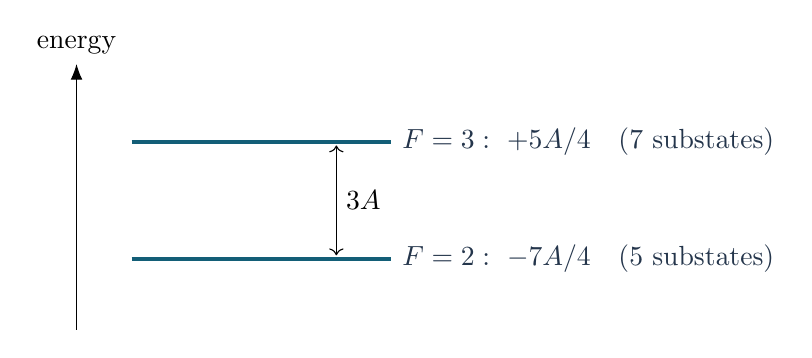
\begin{tikzpicture}[x=1cm,y=.45cm]
\draw[-{Latex[length=2mm]}](0,0)--(0,7.5) node[above]{energy};
\draw[accent,very thick](.7,2)--(4,2) node[right,ink]{\(F=2:\ -7A/4\quad (5~\text{substates})\)};
\draw[accent,very thick](.7,5.3)--(4,5.3) node[right,ink]{\(F=3:\ +5A/4\quad (7~\text{substates})\)};
\draw[<->](3.3,2.1)--(3.3,5.2) node[midway,right]{\(3A\)};
\end{tikzpicture}
\]

\subsection*{(d.i--ii) Weak magnetic field}
For \(\mu_B|B|\ll |A|\) (up to numerical factors),
\(F,m_F\) remain approximately good quantum numbers:
\[
E_{Fm_F}\simeq E_F+\mu_Bg_Fm_FB,\quad
g_F\simeq g_J
\frac{F(F+1)+J(J+1)-I(I+1)}{2F(F+1)}.
\]
For \({}^2P_{1/2}\), \(g_J=2/3\); therefore
\[
\boxed{g_2=-\frac19,\quad g_3=+\frac19.}
\]
The \(F=2\) level becomes \(m_F=-2,-1,0,1,2\)
(5 lines) and \(F=3\) becomes \(-3,\ldots,3\)
(7 lines). Thus generically there are
\(\boxed{12}\) distinct weak-field substates.
Each multiplet fans into equally separated
lines in \(m_F\), but the two multiplets have
opposite slopes.

\subsection*{(d.iii) Strong magnetic field}
When \(\mu_Bg_JB\gg|A|\), the preferred basis is
\(\ket{Jm_J,Im_I}\), with two electronic branches
\(m_J=\pm1/2\), each containing six \(m_I\) values:
\[
E_{m_Jm_I}\simeq
\mu_Bg_Jm_JB+A\,m_Jm_I
\quad\text{(small nuclear Zeeman term neglected)}.
\]
The level pattern looks like two steep
approximately linear electronic fans,
each split by six hyperfine offsets; it is
not appropriate to extrapolate fixed-\(F\) lines
into this regime.

\subsection*{(e) Are higher nuclear multipoles allowed?}
The nuclear spin \(I=5/2\) \emph{can} support a
nuclear electric quadrupole (rank 2), but its
diagonal hyperfine contribution also requires a
rank-2 electronic tensor matrix element
\(\langle J\Vert T^{(2)}\Vert J\rangle\).
By Wigner--Eckart the \(3j\) triangle condition is
\(2\le J+J=1\), which fails for \(J=1/2\).
Thus the \(\boxed{\text{electric-quadrupole hyperfine
term vanishes for this level}}\), as do
higher ranks \(k>1\) at first order within
the fixed \(J=1/2\) manifold.
\solcheck{Total state count:
\(5+7=12=(2I+1)(2J+1)\).
The existence of a nuclear quadrupole alone does
not guarantee a nonzero electronic quadrupole interaction.}

\examquestion{2025}{2}{Ytterbium level diagram, slowing and laser cooling}{3}
The source paper supplies a Yb level diagram, including
\(6s^2\,{}^1S_0\), \(6s6p\ P\) and \(5d6s\ D\) terms.
Distinguish strictly LS-allowed E1 transitions from weak
spin-mixed intercombination lines.
\subsection*{(a) Identify E1 arrows}
Electric dipole (E1) has odd parity and angular rank 1.
In a good LS-coupling approximation, require a parity
change, \(\Delta S=0\), and \(\Delta J=0,\pm1\)
excluding \(0\leftrightarrow0\).
For the terms visible in the supplied diagram,
\[
\begin{array}{l|l}
\text{Level pair}&\text{Strict LS E1?}\\\hline
{}^1P_1\leftrightarrow{}^1S_0&\text{yes}\\
{}^1P_1\leftrightarrow{}^1D_2&\text{yes}\\
{}^3P_1\leftrightarrow{}^3D_1&\text{yes}\\
{}^3P_1\leftrightarrow{}^3D_2&\text{yes}\\
{}^3P_1\leftrightarrow{}^3D_3&\text{no, }\Delta J=2\\
{}^3P_1\leftrightarrow{}^1S_0&
\text{spin-forbidden in pure LS coupling}
\end{array}
\]
With spin--orbit mixing the
\({}^3P_1\leftrightarrow{}^1S_0\) line becomes
a weak \emph{intercombination} E1 transition.
A \(J=0\leftrightarrow0\) line remains forbidden
for a rank-1 operator even with state mixing.
If additional \(P_J\) levels are present in the
original figure, apply the same rules to each.
See the original level diagram in the paper and
the corresponding page preview retained with
the source extractions.

\subsection*{(b) Clock transition}
A clock favours a spectrally narrow, long-lived
transition over a bright, rapidly decaying one.
Among the \(P\) terms visible in the supplied
diagram, one candidate is the much narrower
intercombination transition
\[
\boxed{6s^2\,{}^1S_0\longleftrightarrow
6s6p\,{}^3P_1\quad(\sim556~\mathrm{nm})}.
\]
It is spin-forbidden in pure LS coupling, but
spin--orbit mixing makes it weakly allowed.
This is narrower than the bright
\({}^1S_0\to{}^1P_1\) cooling line and is
a possible frequency reference. The
\emph{standard highest-precision} optical Yb
clock instead uses
\({}^1S_0\leftrightarrow{}^3P_0\) near 578 nm,
a nominally E1-forbidden \(J=0\to0\) line,
in isotopes where it can be interrogated.
Choose that state if it appears in the original
level diagram; either answer must explain
why the chosen excited state is long-lived.

\subsection*{(c) Laser-cooling transition}
Use the strong, nearly cycling
\[
\boxed{6s^2\,{}^1S_0\longleftrightarrow
6s6p\,{}^1P_1\quad(\lambda\simeq399~\mathrm{nm})}.
\]
Its large spontaneous-emission rate allows many
momentum kicks. The narrower
\({}^1S_0\to{}^3P_1\) line near 556 nm
is useful for subsequent cooling.

\subsection*{(d.i) Why the Zeeman slower needs a magnet}
As atoms slow, their Doppler shift changes,
tending to move the laser away from resonance.
A position-dependent magnetic field Zeeman-shifts
the transition and compensates the changing
Doppler shift, maintaining efficient scattering.

\subsection*{(d.ii--iii) Stopping distance and number of photons}
The data are \(M=1.73\times10^{-25}~\mathrm{kg}\),
\(T=300~\mathrm{K}\), \(\lambda=399~\mathrm{nm}\),
and excited-state lifetime \(\tau=5.5~\mathrm{ns}\).
The paper does not specify which characteristic
thermal beam speed to use. Taking the
3D rms speed as an explicit convention,
\[
v_0=\sqrt{\frac{3k_BT}{M}}=
\boxed{268.0~\mathrm{m\,s^{-1}}}.
\]
At saturation a two-level transition has
maximum photon-scattering rate \(\Gamma/2\)
where \(\Gamma=1/\tau\).
Each photon transfers mean directed momentum
\(h/\lambda\), so
\[
F_{\max}=\frac{h}{2\lambda\tau},\quad
a_{\max}=\frac{h}{2M\lambda\tau}.
\]
At \emph{half} the maximum deceleration,
\[
a=\frac{a_{\max}}2
=\frac{h}{4M\lambda\tau}
=\boxed{4.36\times10^5~\mathrm{m\,s^{-2}}}.
\]
Using \(0=v_0^2-2aL\),
\[
\boxed{L=\frac{v_0^2}{2a}=0.0823~\mathrm{m}
=8.23~\mathrm{cm}}.
\]
Momentum balance requires
\[
\boxed{N_\gamma=\frac{Mv_0}{h/\lambda}
=\frac{Mv_0\lambda}{h}\simeq2.79\times10^4}.
\]
If instead one uses the Maxwell most-probable
speed \(\sqrt{2k_BT/M}=218.8~\mathrm{m\,s^{-1}}\),
the corresponding results are
\(L=5.49~\mathrm{cm}\) and
\(N_\gamma\simeq2.28\times10^4\).
State the chosen speed definition in the exam.

\subsection*{(e.i) Red-detuned optical molasses}
An atom moving into a counter-propagating
red-detuned beam sees its light shifted toward
resonance and preferentially absorbs photons
that oppose its motion. The average force near
rest has the form \(\mathbf F\simeq-\beta\mathbf v\).

\subsection*{(e.ii) Doppler limit}
For a simple two-level transition,
\[
T_D=\frac{\hbar\Gamma}{2k_B}
=\frac{h}{4\pi k_B\tau}
=\boxed{6.94\times10^{-4}~\mathrm{K}
=0.694~\mathrm{mK}}.
\]
\solcheck{Cooling requires a bright, rapid
cycling transition; clocks require a narrow,
long-lived one. Check the factor of one-half
in the stated deceleration and the units of
acceleration, length, temperature and photon count.}


\examquestion{2025}{3}{Two-photon NOON input and beam-splitter output probabilities}{4}
With the paper's balanced beam splitter
\(c=(a+b)/\sqrt2,\ d=(a-b)/\sqrt2\), the inverse
relations for creation operators are
\[
a^\dagger=\frac{c^\dagger+d^\dagger}{\sqrt2},
\qquad b^\dagger=\frac{c^\dagger-d^\dagger}{\sqrt2}.
\]
\subsection*{(a) Transform the plus NOON input}
Using \(\ket{2,0}_{ab}=(a^\dagger)^2\ket0/\sqrt2\),
\[
\ket{2,0}\ \longrightarrow\
\frac12\ket{2,0}_{cd}
+\frac1{\sqrt2}\ket{1,1}_{cd}
+\frac12\ket{0,2}_{cd}.
\]
Similarly
\[
\ket{0,2}\ \longrightarrow\
\frac12\ket{2,0}_{cd}
-\frac1{\sqrt2}\ket{1,1}_{cd}
+\frac12\ket{0,2}_{cd}.
\]
The initial state is
\(\ket{\Psi_{\rm in}}=(\ket{2,0}+\ket{0,2})/\sqrt2\).
Add the two output \emph{amplitude vectors}:
\[
\boxed{\ket{\Psi_{\rm out}}=
\frac{\ket{2,0}_{cd}+\ket{0,2}_{cd}}{\sqrt2}}.
\]

\subsection*{(b) Detection probabilities}
Read probabilities from squared moduli:
\[
\boxed{P_{20}=\frac12,\qquad
P_{02}=\frac12,\qquad P_{11}=0}.
\]
They add to 1.

\subsection*{(c) Physical interpretation}
The two input components are \emph{coherent}
number-state amplitudes, so the histories leading
to one photon in each output port interfere
destructively. The input is a two-photon path-entangled
NOON state. The output has perfect two-photon bunching,
but here it originates from the plus-NOON superposition:
this is not the same initial state as the ordinary
two-single-photon HOM experiment. The \emph{minus}
NOON state in the same convention would instead
map to \(\ket{1,1}_{cd}\).

\subsection*{(d) An alternative superposition}
For
\(\ket{\Phi_{\rm in}}=(\ket{1,1}+\ket{2,0})/\sqrt2\),
first transform the \(\ket{1,1}\) part:
\[
a^\dagger b^\dagger\ket0
=\frac{(c^\dagger)^2-(d^\dagger)^2}{2}\ket0
=\frac{\ket{2,0}-\ket{0,2}}{\sqrt2}.
\]
This contains \emph{no} \(\ket{1,1}_{cd}\).
The \(\ket{2,0}\) input contributes
\(\ket{1,1}\) with amplitude \(1/\sqrt2\).
Including the initial superposition coefficient
\(1/\sqrt2\) yields
\[
\boxed{\mathcal A_{11}=\frac12,\qquad
P_{11}=|\mathcal A_{11}|^2=\frac14}.
\]
\solcheck{Never square each path probability before
adding coherent amplitudes; the cancellation in
part (a) would be lost. Account for \(\sqrt{2!}\)
when normalising the two-photon states.}


\examquestion{2025}{4}{Parametric cavity squeezing and entanglement-based random bits}{5}
Start from the supplied quantum Langevin model,
\[
\dot a=-\frac\gamma2a+\sqrt\gamma A_{\rm in},\quad
H_i=\frac{i\hbar\chi}{2}(a^2-a^{\dagger2}).
\]

\subsection*{(a) Derive the modified quantum Langevin equation}
The Heisenberg interaction term is
\(\dot a|_{H_i}=(i/\hbar)[H_i,a]\).
Using \([a^2,a]=0\),
\([a^{\dagger2},a]=-2a^\dagger\), we find
\[
\frac i\hbar[H_i,a]
=\frac i\hbar\frac{i\hbar\chi}{2}(2a^\dagger)
=-\chi a^\dagger.
\]
Thus
\[
\boxed{\dot a=-\chi a^\dagger-\frac\gamma2a
+\sqrt\gamma A_{\rm in}}.
\]

\subsection*{(b) Fourier-domain amplitude quadrature}
Taking the adjoint (real \(\chi\)), and defining
\(X_+=a+a^\dagger\),
\(X_{+,\rm in}=A_{\rm in}+A_{\rm in}^\dagger\),
\[
\dot X_+=-\left(\chi+\frac\gamma2\right)X_+
+\sqrt\gamma X_{+,\rm in}.
\]
Adopt the Fourier convention
\(\tilde X(\omega)=\int e^{-i\omega t}X(t)\diff t\);
then \(\widetilde{\dot X}=i\omega\tilde X\), giving
\[
\boxed{\tilde X_+(\omega)=
\frac{\sqrt\gamma}{\gamma/2+\chi+i\omega}
\tilde X_{+,\rm in}(\omega)}.
\]

\subsection*{(c) Input--output relation}
For the convention \(A_{\rm out}=\sqrt\gamma\,a-A_{\rm in}\),
\[
\tilde X_{+,\rm out}
=\sqrt\gamma\,\tilde X_+-\tilde X_{+,\rm in}
=\left[
\frac{\gamma}{\gamma/2+\chi+i\omega}-1\right]
\tilde X_{+,\rm in}.
\]
Therefore
\[
\boxed{\tilde X_{+,\rm out}=
\frac{\gamma/2-\chi-i\omega}
{\gamma/2+\chi+i\omega}
\tilde X_{+,\rm in}}.
\]
This agrees with the expression requested in the exam.

\subsection*{(d) When does squeezing occur?}
For vacuum input with unit quadrature noise spectrum,
the output \emph{fluctuation spectrum} is
\[
V_+(\omega)=\left|
\frac{\gamma/2-\chi-i\omega}
{\gamma/2+\chi+i\omega}\right|^2
=\boxed{\frac{(\gamma/2-\chi)^2+\omega^2}
{(\gamma/2+\chi)^2+\omega^2}}.
\]
For \(\boxed{0<\chi<\gamma/2}\), the steady
system is below parametric threshold and
\(V_+(\omega)<1\) for finite \(\omega\);
the largest reduction occurs near \(\omega=0\).
The orthogonal quadrature is anti-squeezed.
\begin{cautionbox}
\textbf{Exam notation issue.} The prompt's shorthand
\(V_+=|\langle\tilde X_{+,\rm out}\rangle|^2\)
is not the usual \emph{noise spectral variance}:
for a vacuum input, the mean is zero even though
its fluctuations are nonzero. The physically
relevant squeezing test uses the fluctuation
autocorrelation / power spectrum as above.
\end{cautionbox}

\subsection*{(e) Random and secret bits from Bell pairs}
For \(\ket{\Phi^+}=(\ket{00}+\ket{11})/\sqrt2\),
both parties measuring in the same \(Z\) basis
obtain \(00\) or \(11\), each with probability \(1/2\).
Their local marginal states are maximally mixed:
\(\rho_A=\rho_B=I/2\), hence every local bit is
unpredictable. The outcomes nevertheless match
perfectly. If the pairs are \emph{verified} as
high-fidelity entangled states and Eve is
uncorrelated with them, monogamy limits what
Eve can know. In practice secrecy is not
guaranteed just by \emph{assuming} Bell pairs:
Alice and Bob should estimate disturbance,
authenticate their discussion and perform
error correction/privacy amplification as needed.
\solcheck{The output squeezing factor approaches 1 at
large \(|\omega|\) and is below 1 at \(\omega=0\)
for positive \(\chi\) below threshold.}


\clearpage
\phantomsection
\addcontentsline{toc}{part}{Rapid method index}
\begin{center}{\color{accent}\LARGE\bfseries Rapid method index}
\end{center}
\begin{tabularx}{\linewidth}{@{}p{20mm}X@{}}
\toprule
\textbf{Question}&\textbf{Most reusable starting method}\\\midrule
2023 Q1&Diagonalise \(f(\hat n)\) in Fock basis; expand a
coherent state; inspect parity-dependent phases\\
2023 Q2&Use \(4\pi r^2|\psi|^2\); shell probability and gamma
integrals; enforce fermion antisymmetry/E1 rules\\
2023 Q3&Show optical matrix unitarity; expand output number
difference; compute noise with vacuum input; divide by slope\\
2023 Q4&Enter interaction picture; use spin commutators;
define integrated pulse time; solve Bloch oscillator\\
2024 Q1&Couple \(L,S\to J\); use
\(2\mathbf L\cdot\mathbf S=J^2-L^2-S^2\)\\
2024 Q2&Convert \(\langle\sigma_z\rangle\) to \(P_g\),
differentiate twice; apply dimensions to bias field\\
2024 Q3&Transform creation operators; use normalised Fock
states; compute mean and variance\\
2024 Q4&Fourier transform Langevin equation; apply
input--output relation; keep the loss reservoir\\
2025 Q1&Couple \(I,J\to F\); calculate \(E_F\);
switch from coupled to uncoupled basis at high \(B\)\\
2025 Q2&Test E1 parity/\(\Delta J\)/\(\Delta S\);
scattering \(h/(2\lambda\tau)\); kinematics;
Doppler limit \(\hbar/(2k_B\tau)\)\\
2025 Q3&Expand two-photon creation operators and
sum \emph{amplitudes} before probabilities\\
2025 Q4&Heisenberg commutator; form \(X_+\);
Fourier solve and input--output; noise spectrum\\
\bottomrule
\end{tabularx}
\begin{methodbox}
\textbf{Exam method.} Start by writing the relevant model,
operator definitions and basis. Evaluate symbolically
before numerical substitution. Check probability and
normalisation, limiting cases, angular-momentum
degeneracy, selection-rule triangle/parity conditions
and units. Explain the physical observable in words.
\end{methodbox}
\end{document}
